   
\section[PatternSim]{Метрика основанная на лексико-синтаксических шаблонах}

\subsection{}

\begin{frame}
\frametitle{Публикации}

\begin{itemize}
  \item Hearst, M. A. Automatic acquisition of hyponyms from large text corpora. In ACL,
pages 539–545, 1992. 
\item Panchenko A., Morozova O., Naets H. \textbf{A Semantic Similarity Measure Based on Lexico-Syntactic Patterns.} In Proceedings of KONVENS 2012, pp.174--178, 2012
\item Panchenko A., Romanov P., Morozova O., Naets H., Philippovich A., Fairon
C. \textbf{Serelex: Search and Visualization of Semantically Related Words}.
In Proceedings of the 35th European Conference on Information Retrieval (ECIR 2013).

\item Панченко А., Романов П., Романов А.,  Филиппович А.,
Филиппович Ю., Морозова О. \textbf{Серелекс: поиск и визуализация
семантически связанных слов}. Анализ Изображений, Сетей и Текстов (АИСТ), Интуит, 2013
\end{itemize}
\end{frame}

\begin{frame}
\frametitle{Демо}

\begin{itemize}
  \item {\bf \url{http://serelex.cental.be/} }
  
\begin{figure}  
    \centering
        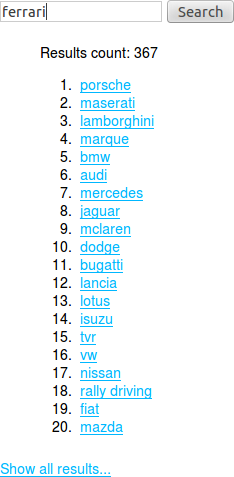
\includegraphics[height=0.6\textwidth]{figures/serelex}
        
\includegraphics[height=0.5\textwidth]{figures/spacer}
        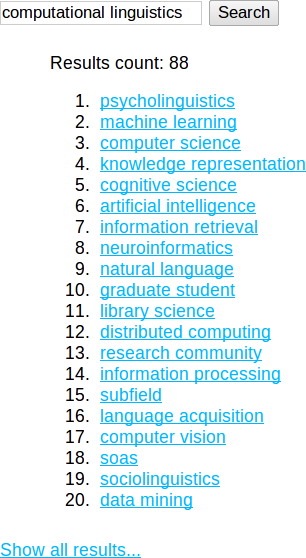
\includegraphics[height=0.6\textwidth]{figures/serelex-2}
        \end{figure}
\end{itemize}
\end{frame}


\begin{frame}
\frametitle{Лексико-синтаксические паттерны}

\begin{itemize}
  \item 18 паттернов извлекающих \textbf{гиперонимы},
  \textbf{ко-гипонимы} и \textbf{синонимы}
\begin{figure}  
    \centering
        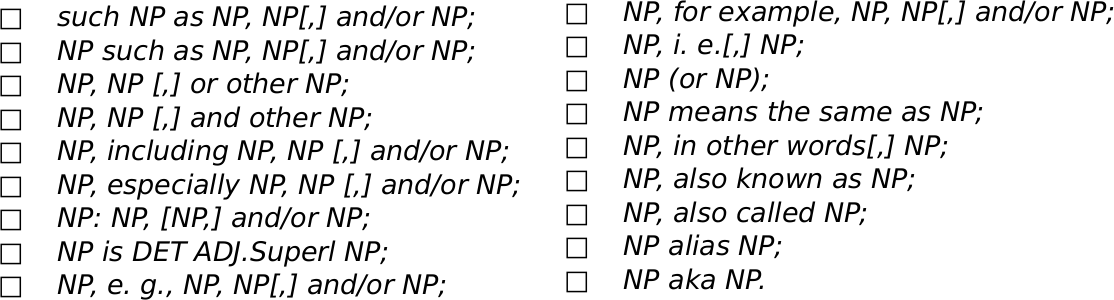
\includegraphics[width=1.0\textwidth]{figures/patterns}
    \end{figure}
\end{itemize}

\end{frame}

\begin{frame}
\frametitle{Основной каскад преобразователей}

\begin{itemize}
  \item Каскад конечных автоматов (FST)
  \item В формате \texttt{Unitex}: \url{http://igm.univ-mlv.fr/~unitex/}
  
\begin{figure}  
    \centering
        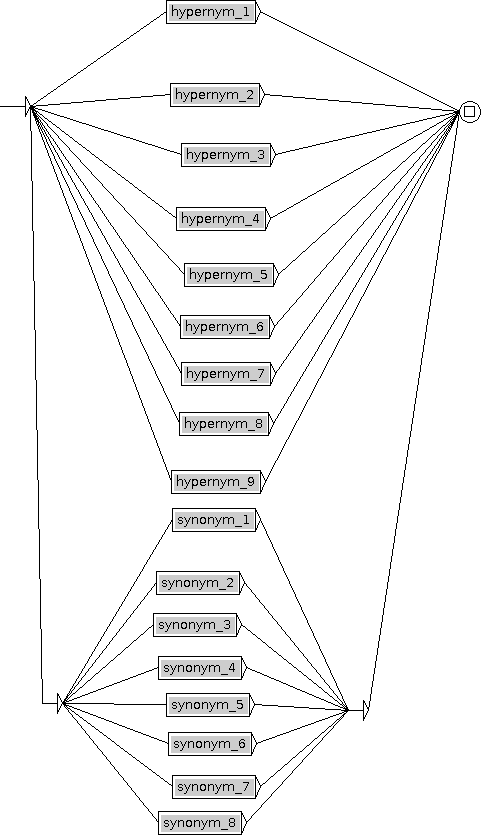
\includegraphics[width=0.3\textwidth]{figures/main-graph}
    \end{figure}
\end{itemize}

\end{frame}

\begin{frame}
\frametitle{Пример реализации паттерна в виде автомата}

\begin{figure}  
    \centering
        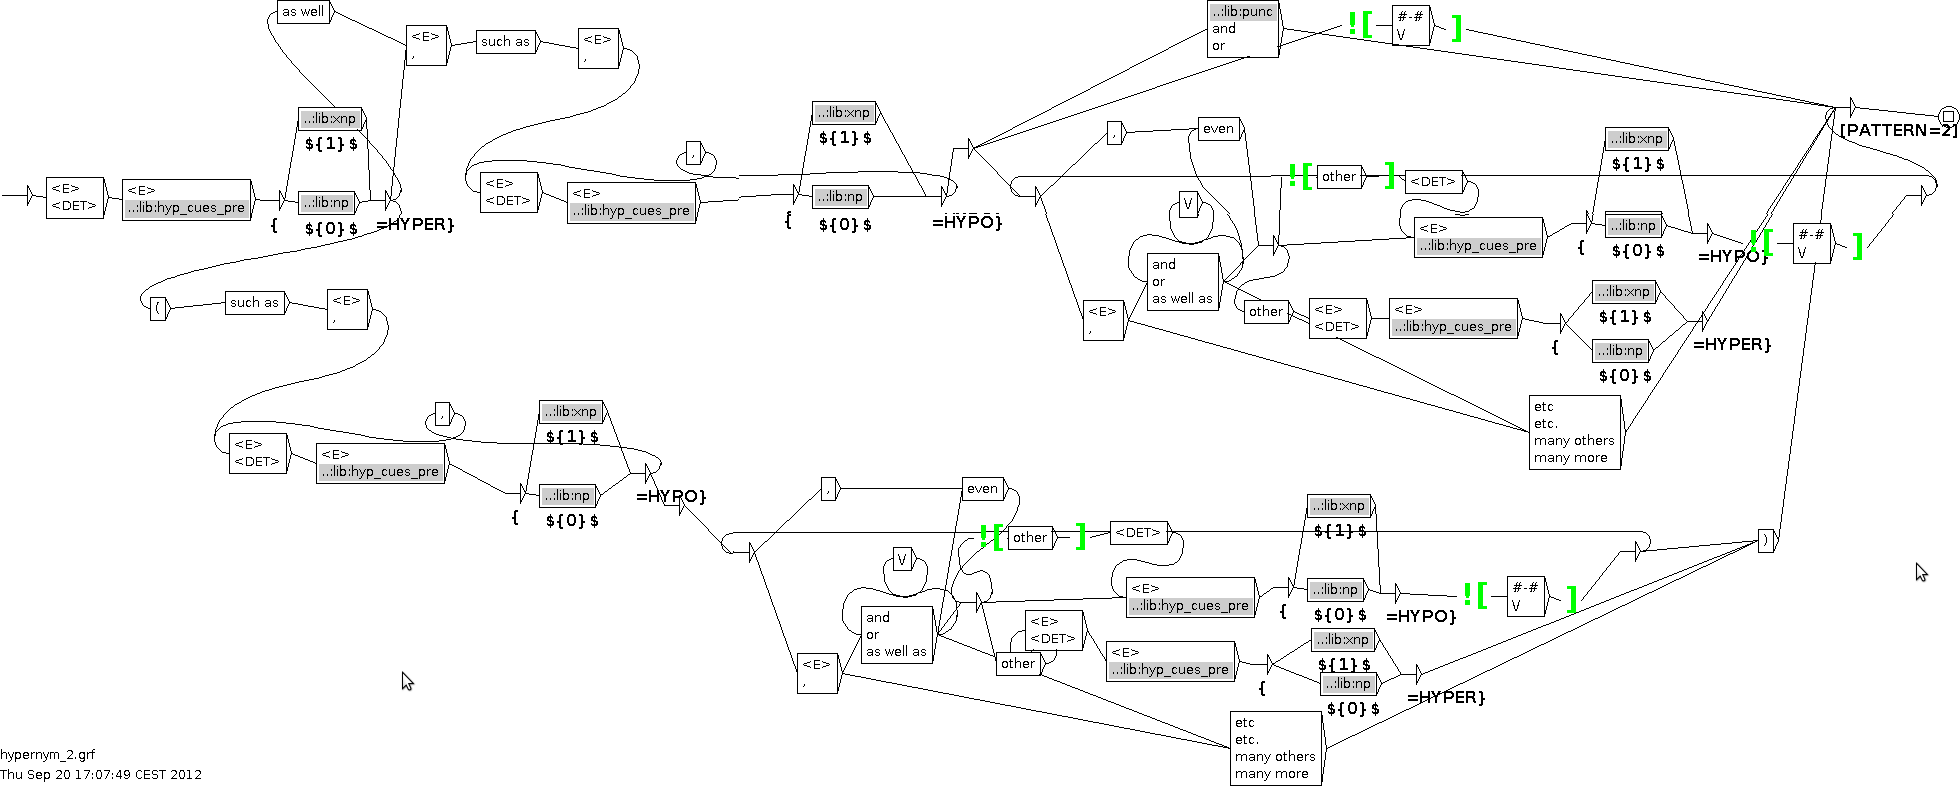
\includegraphics[width=1.0\textwidth]{figures/pattern2}
    \end{figure}

\begin{itemize}
  \item Паттерны, основанные на автоматах позволяют учесть лингвистическую вариацию, сохранив
  точность
      \item В отличие от паттернов основанных на строках (Bollegala et al., 2007)
    
\end{itemize}

\end{frame}






\begin{frame}
\frametitle{PatternSim: основные этапы}


\textbf{Паттерны извлекают конкордансы}

\begin{itemize}
  \item \texttt{such diverse \{[occupations]\} as
  \{[doctors]\}, \{[engineers]\} and \{[scientists]\}[PATTERN=1]}
  \item \texttt{such \{non-alcoholic [sodas]\} as \{[root beer]\} and \{[cream soda]\}[PATTERN=1]}
  \item \texttt{\{traditional[food]\}, such as \{[sandwich]\},\{[burger]\}, and \{[fry]\}[PATTERN=2]}
\end{itemize}

\end{frame}






\begin{frame}
\frametitle{PatternSim: основные этапы}

\textbf{Корпус} Wikipedia+ukWaC: $2.9\cdot10^{12}$ токенов

\begin{figure}  
\centering
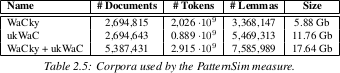
\includegraphics[width=0.7\textwidth]{figures/patternsim-table}
\end{figure}


\textbf{Количество извлечений}

\begin{itemize}
  \item Wikipedia -- 1.196.468 
  \item ukWaC -- 2.227.025 
  \item WaCypedia+ukWaC -- 3.423.493
\end{itemize}

\end{frame}





\begin{frame}
\frametitle{Метрика семантической близости PatternSim }

\begin{figure}  
\centering
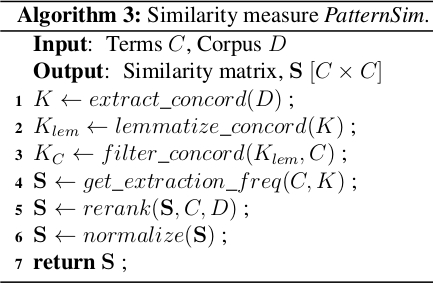
\includegraphics[width=0.6\textwidth]{figures/patternsim-algo}
\end{figure}

\end{frame}



\begin{frame}
\frametitle{Вычисление подобия: rerank}


\begin{itemize}
  \item \textbf{Efreq}: мера подобия равна количеству извлеченных отношений
  $$ s_{ij} = s_{ij} $$
  
  \item \textbf{Efreq-Cfreq}: нормализация по частоте слов
  
  $$ s_{ij} = \frac{P(c_i,c_j)}{P(c_i)P(c_j)} $$ 
    
    \begin{itemize}
    \item $P(c_i,c_j)=\frac{e_{ij}}{\sum_{ij}e_{ij}}$ -- вероятность извлечения
отношения $\langle c_i,c_j \rangle$, где $e_{ij}$ -- частота
взаимной встречаемости слов $c_i$ и $c_j$ во множестве конкордансов

\item $P(c_i)= \frac{f_i}{\sum_i f_i}$ -- вероятность слова $c_i$, где $f_i$
-- частота $c_i$

\end{itemize}
    
\end{itemize}

\end{frame}


\begin{frame}
\frametitle{Вычисление подобия: }
  
\begin{itemize}
  
\item \textbf{Efreq-Rnum-Cfreq-Pnum}:
  
$$s_{ij} = \sqrt{p_{ij}} \cdot \frac{2\cdot\mu_b }{b_{i*}+b_{*j}} \cdot \frac{P(c_i,c_j)}{P(c_i)P(c_j)}.$$

\begin{itemize}

\item $P(c_i,c_j)=\frac{e_{ij}}{\sum_{ij}e_{ij}}$ -- вероятность извлечения
отношения $\langle c_i,c_j \rangle$, где $e_{ij}$ -- частота
взаимной встречаемости слов $c_i$ и $c_j$ во множестве конкордансов

\item $P(c_i)= \frac{f_i}{\sum_i f_i}$ -- вероятность слова $c_i$, где $f_i$
-- частота $c_i$
\item $b_{i*} = \sum_{j:e_{ij} \geq \beta} 1$ -- количество извлечений слова
$c_i$ с частотой $\geq \beta$,  где $\mu_b = \frac{1}{|C|}\sum_{i=1}^{|C|}
b_{i*}$ -- среднее количество извлечений для отдельного слова

\item $p_{ij} \in [1;18]$ -- количество отдельных паттернов которые извлекли
отношение $\langle c_i, c_j \rangle$
 
\end{itemize}
\end{itemize}

\end{frame}






\begin{frame}
\frametitle{Ранжирование семантических отношений}

\begin{itemize}
  \item Точность \textbf{сравнима или лучше} чем у аналогов;
  \item Полнота \textbf{меньше} чем у аналогов.
\end{itemize}

\begin{figure}  
    \centering
    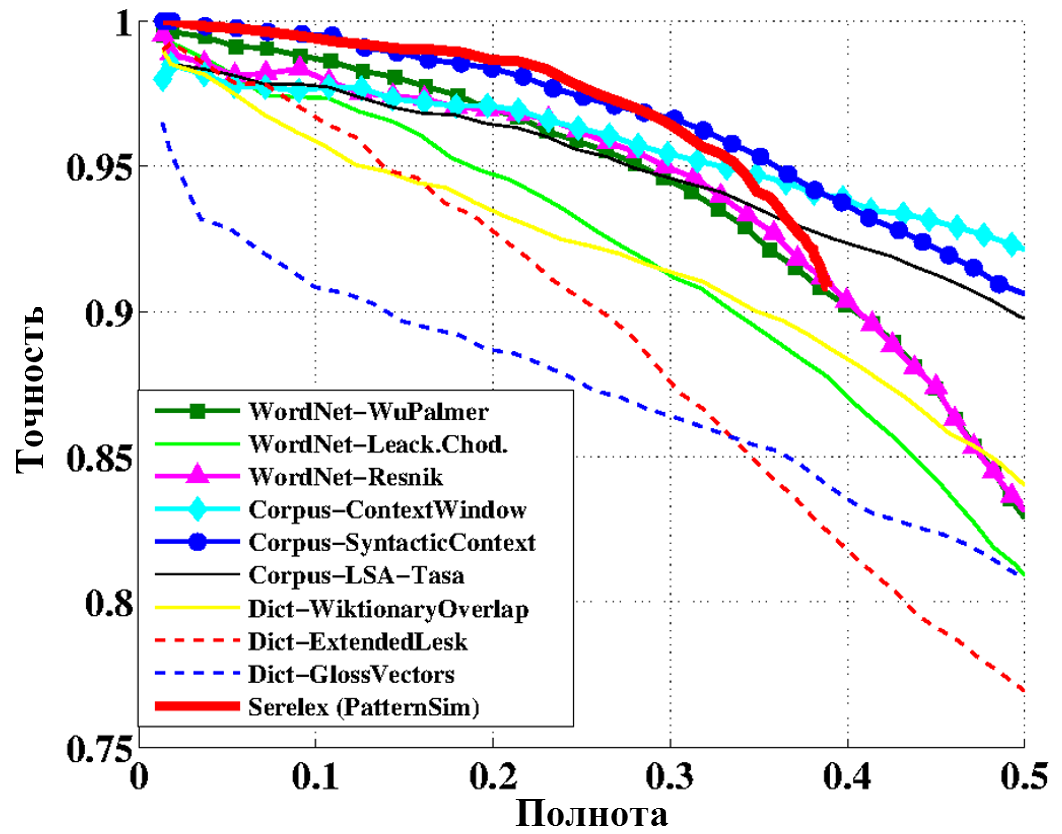
\includegraphics[width=0.6\textwidth]{pr}
    \caption{График точность-полнота (коллекция BLESS).
    }
\end{figure}

\end{frame}








\begin{frame}
\frametitle{Извлечение семантических отношений}
  \begin{columns}[T]
    \begin{column}{.4\textwidth}
     
% Your text here
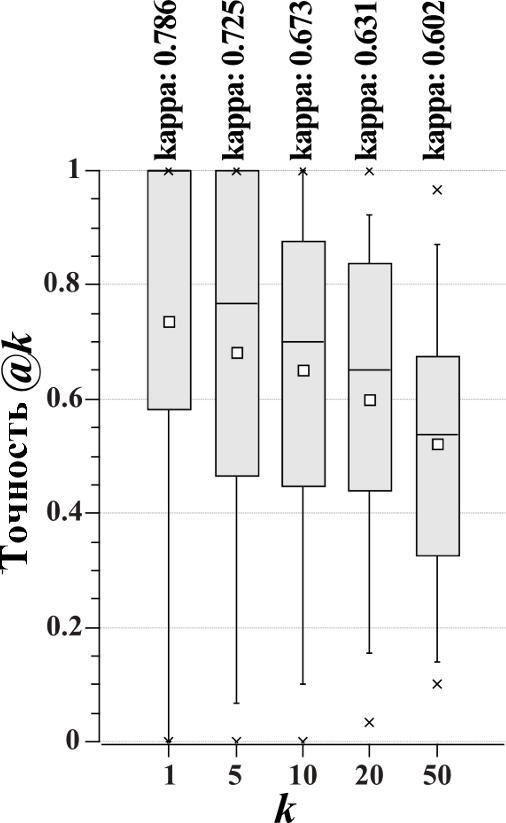
\includegraphics[width=0.85\textwidth]{./kappa}
    
    \end{column}
    \begin{column}{.6\textwidth}
    %\begin{block}{Your image}
\begin{itemize}
  %\item 49 words, three binary annotations;
  \item Точность@1 $\approx 0.80$;
  \item ``Хорошее'' лексическое покрытие:
  
\end{itemize}

\begin{figure}
\includegraphics[width=0.95\textwidth]{./../figures/wordnet-vs-serelex}
\end{figure}
      
    \end{column}
  \end{columns}
\end{frame}






\begin{frame}
\frametitle{Сравнение результатов базовых метрик и PatternSim}

\begin{figure}  
\centering
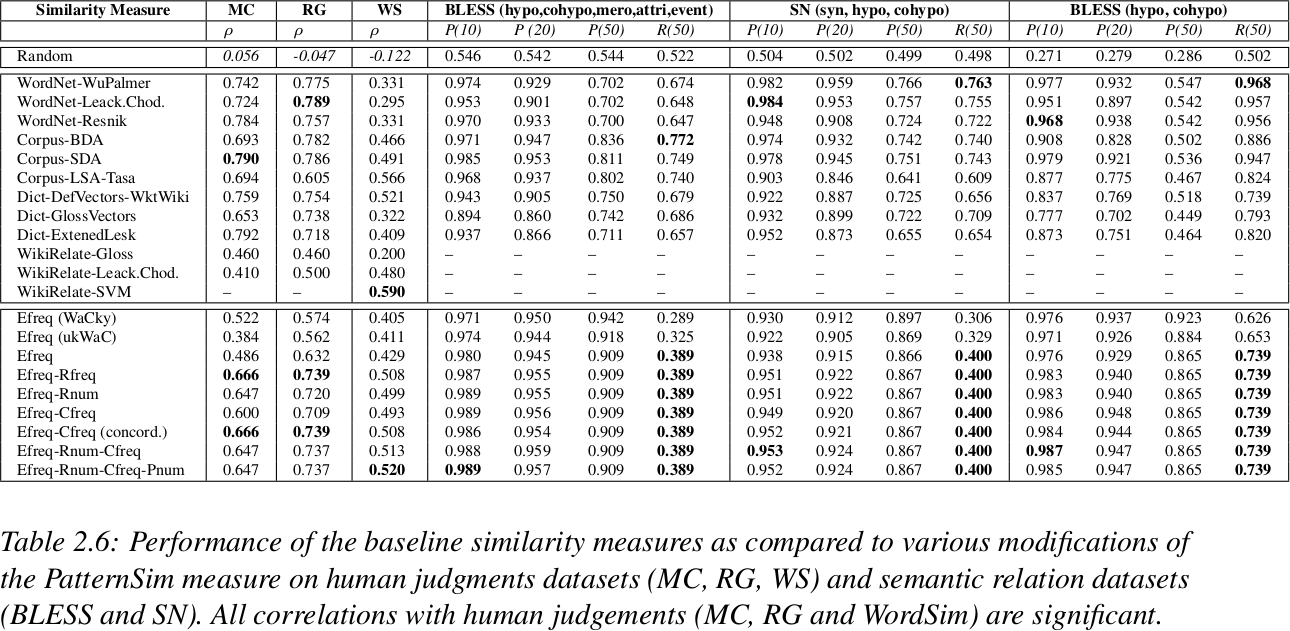
\includegraphics[width=0.9\textwidth]{figures/patternsim-results-table}
\end{figure}

\end{frame}


